\chapter{Revisão Bibliográfica}
\label{cap:02}

Neste capítulo, será feita uma revisão da fundamentação teórica necessária utilizada ao longo deste projeto, visando alcançar o objetivo proposto. % apresentação genérica

\section{Inteligência Artificial}

A inteligência artificial é uma área de estudo da ciência da computação que busca compreender e simular a inteligência humana a fim de reproduzi-la artificialmente em uma máquina \cite{Haugeland1985}. Ela envolve o uso de algoritmos, sistemas e técnicas que permitem que as máquinas aprendam e realizem tarefas que normalmente exigiriam a inteligência humana.

Para desenvolver a IA, usamos técnicas que se associam as funções cognitivas da mente humana. Como o uso de redes neurais que buscam replicar o funcionamento dos neurônios no cérebro humano. O aprendizado de máquina, que treina computadores para desempenhar tarefas semelhantes às realizadas por seres humanos. Isso inclui as habilidades como planejamento, compreensão, aprendizado, raciocínio, resolução de problemas e tomada de decisões com base em dados e informações fornecidas.

A IA é um campo multidisciplinar que combina conhecimentos da ciência da computação, da matemática, da estatística, da neurociência e de outras áreas para criar programas e sistemas capazes de aprender, raciocinar, reconhecer padrões, tomar decisões e resolver problemas de forma autônoma. Existem diferentes abordagens, técnicas e aplicações da inteligência artificial, mas o aprendizado de máquina é uma das bases fundamentais para seu funcionamento e, consequentemente, para realização deste trabalho.

\section{Aprendizado de Máquina}

O aprendizado de máquina é uma aplicação na qual os sistemas são treinados com grandes conjuntos de dados para reconhecer padrões, fazer previsões e tomar decisões com base nesses padrões \cite{HoschMachineLearning}. Trata-se de um método de análise de dados que utiliza uma abordagem estatística e computacional, permitindo que os sistemas aprendam com os dados disponíveis e com o mínimo de intervenção humana necessária, um exemplo é a moderação do conteúdo postado em redes sociais, com a finalidade de classificar se um determinado conteúdo é ofensivo ou não.

Existem várias abordagens de aprendizado de máquina, sendo o aprendizado supervisionado, as redes neurais, o \textit{deep learning} e o aprendizado por conjuntos de grande importância para a execução deste trabalho.

\subsection{Aprendizado supervisionado}

O aprendizado supervisionado utiliza um conjuntos de dados rotulados para treinar algoritmos com o objetivo de aprender a classificar os dados ou prever resultados com precisão com base nas informações fornecidas nos rótulos dos dados de treinamento. O modelo realiza ajustes finos (do inglês, \textit{fine-tuning}) à medida que os dados de entrada são inseridos, visando aprender a mapear corretamente os dados para as saídas desejadas. Isso permite a previsão ou classificação de novos exemplos não rotulados com base no aprendizado adquirido \cite{RussellNorvig1995}.

\subsection{Redes Neurais}

As redes neurais são uma analogia neurobiológica inspirada no funcionamento do sistema nervoso do cérebro humano, capazes de adquirir conhecimento através de um processo de aprendizagem a partir de dados de entrada, com ou sem supervisão. Essas redes são capazes de armazenar o conhecimento adquirido interligando células computacionais simples denominadas ``neurônios'' ou ``unidades de processamento''. Com essa estrutura interconectada, e com o treinamento apropriado, são capazes de modelar, analisar e reconhecer padrões, resultando na produção de conhecimento de maneira distribuída \cite{Haykin2007}.

\begin{figure*}[!htbp]
	\centering
	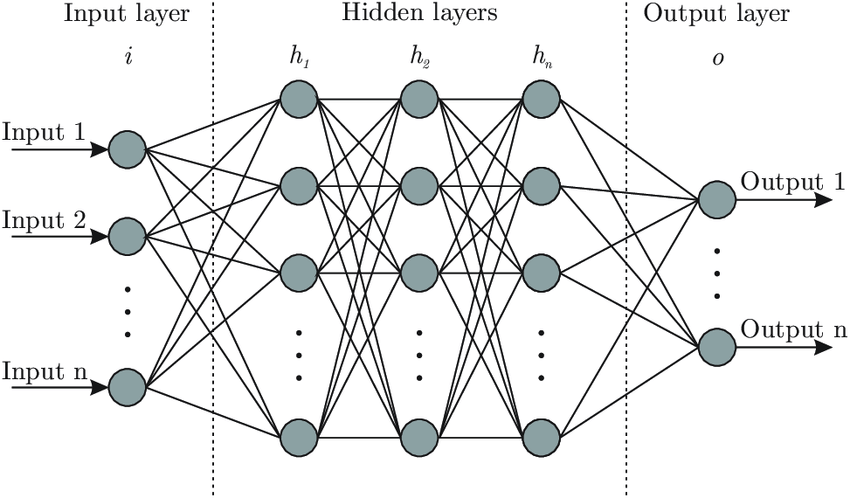
\includegraphics[scale=0.4]{imagens/arch-rede-neural-artificial.png}
    \caption {Arquitetura de uma Rede Neural Artificial \cite{RedeNeuralImagem}.}
\end{figure*}

Elas são compostas por um conjunto interconectado de neurônios artificiais, ou ``nós'', que são organizados em várias camadas, sendo a de entrada responsável por receber os dados, as intermediárias (também conhecidas como camadas ocultas) responsáveis por processar as informações e a de saída responsável por produzir as saídas finais com os resultados da rede neural.

Cada neurônio artificial possui pesos e um valor de viés, sendo o primeiro representando a importância da conexão entre os neurônios, enquanto o segundo é uma medida flexível que facilita a ativação do neurônio de acordo com as preferências incorporadas. Durante o treinamento, os pesos e vieses são ajustados para otimizar o desempenho da rede. A rede funciona por meio de dois processos principais, a propagação direta (do inglês, \textit{forward propagation}), e a retropropagação do erro (do inglês, \textit{backpropagation}). Na propagação direta, os dados de entrada são alimentados na rede neural, passando pelos neurônios e pelas camadas, e resultando em uma saída. Cada neurônio combina linearmente os valores de entrada ponderados pelos pesos, aplica uma função de ativação e repassa o resultado para os neurônios da próxima camada. O erro é calculado em relação aos valores desejados, e a retropropagação do erro ajusta os pesos e vieses dos neurônios para minimizar o erro. Esse processo é repetido até que os pesos sejam ajustados para produzir resultados desejáveis.

Elas são amplamente utilizadas em áreas como visão computacional e processamento de linguagem natural devido à sua capacidade de aprender a partir dos dados e fornecer soluções complexas para problemas desafiadores, capazes de extrair características relevantes dos dados e realizar tarefas como classificação e reconhecimento de padrões.

\subsection{Aprendizado profundo}

O aprendizado profundo (do inglês, \textit{deep learning}) é uma abordagem que utiliza redes neurais artificiais profundas que utilizam múltiplas camadas de processamento interconectadas para extrair representações complexas dos dados com vários níveis de abstração e reconhecimento de padrões. Essas redes neurais profundas são capazes de aprender de forma hierárquica, com cada camada representando características mais abstratas à medida que se aprofunda na rede \cite{AurelienGeron2019}. Essa abordagem permite que o aprendizado profundo seja capaz de lidar com problemas de maior complexidade e extraia automaticamente características relevantes dos dados.

O aprendizado profundo e as redes neurais tem impulsionado significativamente o avanço em áreas como a visão computacional e o processamento de linguagem natural.

\subsection{Aprendizado por conjuntos}

O aprendizado por conjuntos (do inglês, \textit{ensemble learning}) é uma técnica que combina múltiplos modelos de aprendizado de máquina para melhorar o desempenho e a precisão das previsões \cite{OPITZEnsemble}. Ao invés de depender de um único modelo, o aprendizado por conjuntos aproveita a diversidade e a opinião coletiva dos modelos individuais para tomar decisões mais precisas, pois os erros cometidos por um modelo podem ser compensados por outros mais precisos. 

Uma abordagem comum no \textit{ensemble learning} é o \textbf{voto majoritário}, em que cada modelo do conjunto faz uma previsão para uma determinada instância de dados, conhecida como classe, e a classe mais frequente entre os modelos é escolhida como a previsão final. O voto majoritário é simples e eficaz, especialmente quando os modelos individuais têm uma taxa de acerto significativa. Outras estratégias também podem ser utilizadas, como a combinação de probabilidades ou o uso de pesos para ponderar as previsões dos modelos individuais. Essas abordagens levam em consideração a confiança ou a qualidade dos modelos, o que contribui para um aumento geral na precisão das previsões.

Outra abordagem importante de destacar é o uso dos \textbf{hiperparâmetros}, que são parâmetros configuráveis que afetam o desempenho e o comportamento do modelo, influenciando fatores como a complexidade, a velocidade de treinamento e a capacidade de generalização. No \textit{ensemble learning}, os hiperparâmetros são usados para selecionar os modelos de melhor desempenho para o conjunto por meio da busca em grade, que envolve uma grade de valores de hiperparâmetros onde é feita a pesquisa de todas as combinações possíveis desses valores. A seleção adequada dos hiperparâmetros é fundamental para otimizar o desempenho do \textit{ensemble learning} e obter os melhores resultados, da qual requer ajustes dos valores dos hiperparâmetros e avaliação do desempenho do modelo usando métricas apropriadas. Tais métricas são essenciais para avaliar e mensurar os resultados obtidos, sendo elas a acurácia e a AUROC.

A \textbf{acurácia} é uma métrica que avalia a performance de um modelo de aprendizado de máquina, representando a proporção de previsões corretas em relação ao total de previsões realizadas pelo modelo. É calculada dividindo o número de previsões corretas pelo número total de exemplos no conjunto de dados. No entanto, em casos de desbalanceamento de dados, quando uma classe é mais frequente que as outras, a acurácia por si só não é a métrica mais adequada. Nesses casos, é importante considerar outras métricas que possam fornecer uma visão mais abrangente do desempenho do modelo, como a AUROC.

A \textbf{AUROC} (Área sob a Curva Característica de Operação do Receptor) é uma métrica utilizada principalmente para avaliar o desempenho de modelos de classificação binária, como os utilizados em problemas de detecção de conteúdo ofensivo ou não. A curva ROC (Característica de Operação do Receptor) é construída traçando a taxa de verdadeiros positivos em relação à taxa de falsos positivos para diferentes pontos de corte de classificação. A AUROC é a área sob essa curva, variando de 0 a 1, onde um valor mais próximo de 1 indica um modelo com melhor capacidade de distinguir entre as classes. Em geral, uma AUROC de 0,5 indica um modelo com desempenho aleatório, enquanto valores acima de 0,5 indicam um desempenho melhor do que o aleatório \cite{BradleyAUROC}.

\begin{figure*}[!htbp]
	\centering
	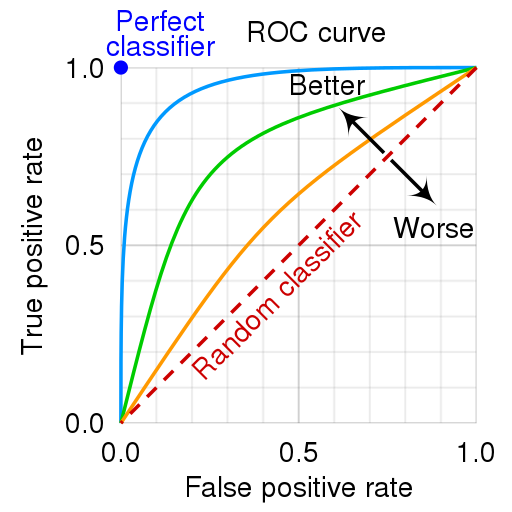
\includegraphics[scale=0.36]{imagens/auroc.png}
    \caption {Curva ROC para um classificador ``melhor'' e ``pior'' \cite{RocCurveWiki}.}
\end{figure*}

O \textit{ensemble learning} é uma técnica amplamente adotada para melhorar a precisão e a estabilidade dos modelos de aprendizado de máquina, frequentemente utilizada em problemas do mundo real, onde a precisão é crucial.

\section{Processamento de Linguagem Natural}

O processamento de linguagem natural (PLN) é uma subárea da inteligência artificial e da linguística que estuda a compreensão e geração automática da linguagem humana. Os sistemas de geração de linguagem natural convertem informação armazenadas em bancos de dados computacionais em linguagem compreensível ao ser humano, enquanto os sistemas de compreensão de linguagem natural convertem ocorrências da linguagem humana em representações mais formais, mais facilmente manipuláveis por programas de computador. O PLN abrange uma variedade de tarefas, como a tradução e geração de respostas automáticas, sumarização de texto, reconhecimento de fala, análise de sentimento, que busca extrair qualidades subjetivas – emoções, humor, sarcasmo, ofensa, motivação, confusão – do texto e muito mais. O objetivo principal do PLN é permitir que os computadores compreendam, interpretem e gerem texto e fala de forma semelhante a linguagem humana\footnote{\textit{What is Natural Language Processing?} | IBM. Disponível em: \url{https://www.ibm.com/topics/natural-language-processing}. Acesso em: 12 de jun. de 2023.}.

Atualmente, os modelos de aprendizagem profunda e as técnicas baseadas em redes neurais possibilitam sistemas de PLN serem capazes de aprender e extrair significados cada vez mais precisos de grandes quantidades de texto bruto. Esses sistemas têm a capacidade de aprimorar seu desempenho à medida que trabalham, permitindo uma compreensão mais avançada da linguagem natural, como os \textit{transformers}.

\subsection{\textit{Transformers}}

Os \textit{transformers} são uma arquitetura de rede neural profunda que revolucionaram o campo do processamento de linguagem natural. Ao contrário das redes neurais convencionais, os \textit{transformers} têm a capacidade de processar informações de uma sequência de entrada de forma simultânea, em vez de depender de um processamento sequencial. Isso permite uma maior paralelização, uma melhor compreensão do contexto global do texto e, consequentemente, uma redução do tempo de treinamento, o que resulta em uma melhoria significativa na eficiência em comparação com as redes neurais tradicionais \cite{GoogleTeamTransformers}. Isso é possível graças ao mecanismo de atenção, que permite que cada elemento da sequência interaja com todos os outros, fornecendo contexto relevante. Os \textit{transformers} têm sido amplamente adotados e são considerados o estado da arte\footnote{\textit{state-of-the-art}. Disponível em: \url{https://www.oxfordlearnersdictionaries.com/definition/english/state-of-the-art}. Acesso em: 12 de jun. de 2023.} no processamento de linguagem natural. Essa designação se refere à abordagem mais avançada e eficaz atualmente disponível no campo do processamento de linguagem natural, baseada em resultados de pesquisa, no desempenho superior em comparação com outras abordagens e na validação em estudos científicos e aplicações práticas.

A arquitetura dos \textit{transformers} é composta por um codificador e um decodificador, ambos contendo várias camadas. O \textbf{codificador} recebe uma sequência de entrada e gera uma representação contextualizada dessa sequência, é responsável por capturar as informações relevantes e as relações entre as palavras ou elementos da sequência. Por sua vez, o \textbf{decodificador} utiliza a representação contextual gerada pelo codificador juntamente com uma sequência de referência para gerar uma sequência de saída, é responsável por produzir a saída desejada com base no contexto e nas informações disponíveis. Ambos utilizam os mecanismos de atenção, autoatenção (do inglês, \textit{self-attention}), atenção de múltiplas cabeças (do inglês \textit{multi-head attention}) e a rede \textit{feed-foward}.

A ``atenção'' é um mecanismo fundamental no processamento de sequências, ela permite que um modelo se concentre em partes relevantes de uma sequência ao ponderar a importância de cada elemento em relação aos outros, calculando sua importância em relação a todos os outros elementos, resultando em uma matriz de pesos de atenção. Já a \textbf{autoatenção} em vez de comparar cada elemento com todos os outros, ela calcula as interações entre os elementos dentro da mesma sequência. Isso é feito por meio de transformações lineares e funções de similaridade, como o a função \textit{softmax}. A autoatenção permite que cada elemento da sequência se relacione com todos os outros elementos, capturando informações contextuais e de dependência importantes. 

Por sua vez, a atenção de múltiplas cabeças permite que o modelo capture informações contextuais de diferentes perspectivas, dividindo a representação de entrada em várias ``cabeças'', cada uma responsável por calcular pesos de atenção que indicam a importância relativa das palavras em relação umas às outras. Os valores são então combinados de acordo com os pesos de atenção, resultando em uma representação ponderada das palavras, que captura relações complexas e melhora a capacidade de representação e aprendizado dos \textit{transformers}.

Por fim, a rede \textit{feed-forward} é um tipo de rede neural, composta por duas camadas lineares com uma função de ativação não linear aplicada entre elas, que é executada individualmente a cada posição na sequência de entrada de forma idêntica. Seu objetivo é fornecer uma transformação não linear que captura padrões complexos e dependências entre os elementos da sequência. Ao introduzir a não linearidade e aprender padrões não lineares, a rede \textit{feed-forward} possibilita que o \textit{transformer} capte informações contextuais e complexas em cada posição da sequência. Isso contribui para a capacidade do modelo de processar efetivamente o contexto da linguagem natural e melhorar o desempenho.

\begin{figure*}[!htbp]
	\centering
	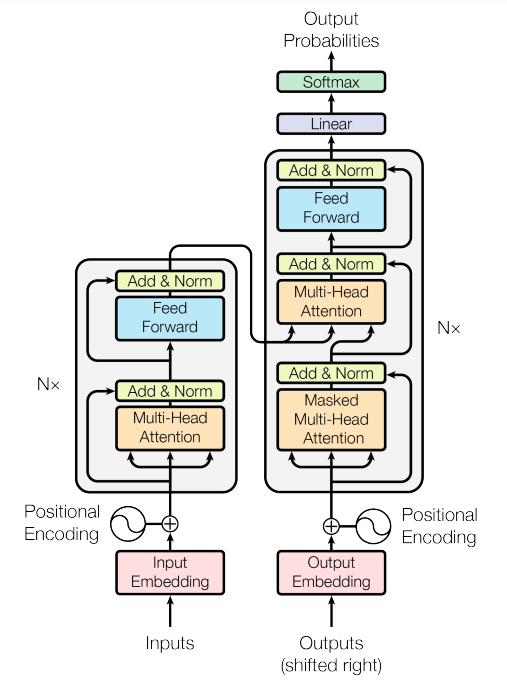
\includegraphics[scale=0.6]{imagens/arch-transformers.png}
    \caption {Modelo de arquitetura de um \textit{transformer} \cite{GoogleTeamTransformers}.}
\end{figure*}

Os \textit{transformers} têm sido amplamente adotados em várias aplicações de PLN e até mesmo em outros domínios, devido à sua capacidade de lidar com sequências de texto de comprimento variável, aprender representações contextualizadas e gerar previsões precisas. Comparados aos modelos de redes neurais, os transformadores são mais receptivos à paralelização, permitindo o treinamento em conjuntos de dados maiores. Isso levou ao desenvolvimento de sistemas pré-treinados, como o BERT e o GPT, que foram treinados com grandes conjuntos de dados de linguagem. Além disso, os \textit{transformers} têm mostrado sucesso não apenas no processamento de linguagem natural, mas também em outras áreas, como visão computacional.

\subsection{BERT}

O BERT (do inglês, \textit{Bidirectional Encoder Representations from Transformers}) é um modelo de linguagem pré-treinado desenvolvido pela \citeonline{BERTImagem}, baseado na arquitetura do \textit{transformer}. Foi treinado em uma grande quantidade de dados não rotulados para aprender representações ricas e contextuais das palavras. O treinamento do BERT envolve duas tarefas principais: ``previsão de máscara'' e ``próxima sentença''. Na previsão de máscara, palavras em uma sequência de texto são mascaradas e o modelo é treinado para prever as palavras mascaradas com base no contexto. Na tarefa de próxima sentença, o BERT aprende a prever se duas sentenças são sequenciais ou não.

O BERT alcançou resultados significativos em várias tarefas de processamento de linguagem natural quando combinado com tarefas de ajuste fino em conjuntos de dados específicos. Ao pré-treinar o modelo em grandes quantidades de dados e depois ajustá-lo para tarefas específicas, o BERT é capaz de capturar nuances semânticas e sintáticas das palavras, melhorando o desempenho em classificação de texto, resposta a perguntas, sumarização e muito mais.

\begin{figure*}[!htbp]
	\centering
	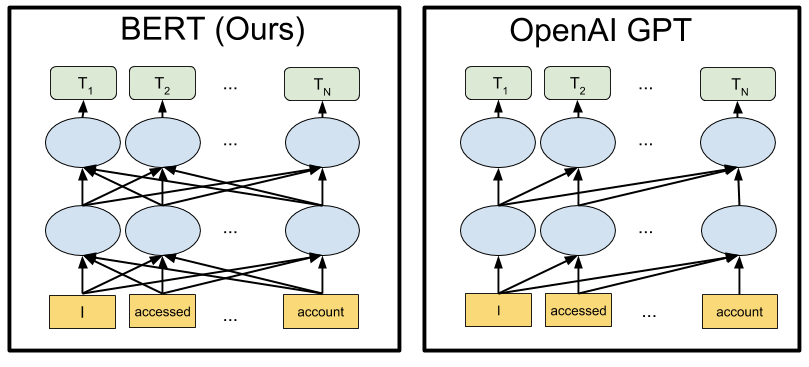
\includegraphics[scale=0.4]{imagens/BERT.png}
    \caption {Representação do BERT (bidirecional), e da OpenAI GPT (unidirecional) \cite{BERTImagem}.}
\end{figure*}

O diferencial do BERT em relação a outros modelos de linguagem pré-treinados é a sua capacidade bidirecional de compreender o contexto das palavras, considerando o contexto anterior e posterior de cada palavra ao realizar o seu processamento, o que permite ao modelo uma melhor compreensão do significado das palavras e frases em um texto, levando em conta as dependências entre elas. Os resultados mostram que modelos de linguagem treinados de forma bidirecional, como o BERT, fornecem uma compreensão mais profunda do contexto linguístico do que os modelos unidirecionais.

\section{Visão Computacional}

A visão computacional é uma área de estudo e aplicação da inteligência artificial que busca capacitar os computadores a interpretarem, analisarem e compreenderem o conteúdo visual de imagens ou vídeos de maneira similar ao ser humano. Isso envolve o desenvolvimento de algoritmos e técnicas que permitem que os sistemas computacionais obtenham informações úteis a partir de dados visuais, e realizem tarefas como reconhecimento facial e de objetos, detecção de padrões, análise de expressões faciais, classificação automática de imagens em redes sociais entre outros\footnote{\textit{What is Computer Vision?} | IBM. Disponível em: \url{https://www.ibm.com/topics/computer-vision}. Acesso em: 12 jun. 2023.}.

A integração de técnicas de visão computacional com outros campos, como processamento de linguagem natural, tem impulsionado pesquisas e avanços significativos na análise e compreensão de dados visuais. Essa integração tem permitido a aplicação de técnicas avançadas de processamento de linguagem natural no campo da visão computacional, resultando em melhorias nas tarefas relacionadas à interpretação e compreensão de informações visuais, como o \textit{VisualBERT}.

\subsection{\textit{VisualBERT}}

O \textit{VisualBERT} é um modelo de linguagem pré-treinado que combina processamento de linguagem natural e a visão computacional para entender e interpretar informações visuais e textuais simultaneamente, baseado na arquitetura do BERT, ao contrário dos modelos que se baseiam apenas em texto, ele incorpora também representações visuais das imagens para melhorar o desempenho em tarefas que envolvem texto e contexto visual. O modelo é treinado em um grande conjunto de dados multimodais que combina texto descritivo e imagens correspondentes, tal abordagem permite que o \textit{VisualBERT} capture informações visuais relevantes, permitindo uma melhor compreensão de textos relacionados a imagens e aprimorando o desempenho em tarefas como descrição de imagens, geração de legendas entre outros. O \textit{VisualBERT} representa uma extensão dos modelos de linguagem pré-treinados, integrando efetivamente a visão computacional ao processamento de linguagem natural para uma análise mais completa e precisa de conteúdos multimodais \cite{VisualBERTArt}.

O \textit{VisualBERT} é pré-treinado usando dois objetivos semelhantes aos usados no BERT: modelagem de linguagem mascarada com previsão de alinhamento de imagens e legendas. O processo de pré-treinamento envolve treinar o modelo com um grande conjunto de dados multimodais que combinam texto descritivo e imagens correspondentes, para prever alguma parte oculta (mascarada) da entrada, seja uma parte de uma imagem ou uma palavra do texto. Após o pré-treinamento, o modelo passa por um processo de ajuste fino em conjuntos de dados específicos para aprimorar seu desempenho. Isso permite que o modelo se adapte às características e nuances das tarefas específicas, refinando ainda mais suas representações multimodais.

A arquitetura do \textit{VisualBERT} utiliza uma camada de entrada compartilhada para codificar tanto o texto quanto as representações visuais. Utilizando técnicas de codificação de palavras e redes neurais, essa camada captura informações contextuais das palavras e das representações visuais por meio de várias camadas do codificador do \textit{transformer}, assim como o BERT. Cada camada do codificador possui subcamadas de atenção \textit{multi-head} e redes \textit{feed-forward}, permitindo a captura de interações e padrões entre palavras e informações visuais. Os recursos visuais extraídos das propostas de objetos são tratados como \textit{tokens} de entrada não ordenados e incorporados no \textit{VisualBERT} juntamente com o texto. Essa abordagem permite que o modelo capture e relacione informações tanto textuais quanto visuais, permitindo uma compreensão mais completa dos dados multimodais.

\begin{figure*}[!htbp]
	\centering
	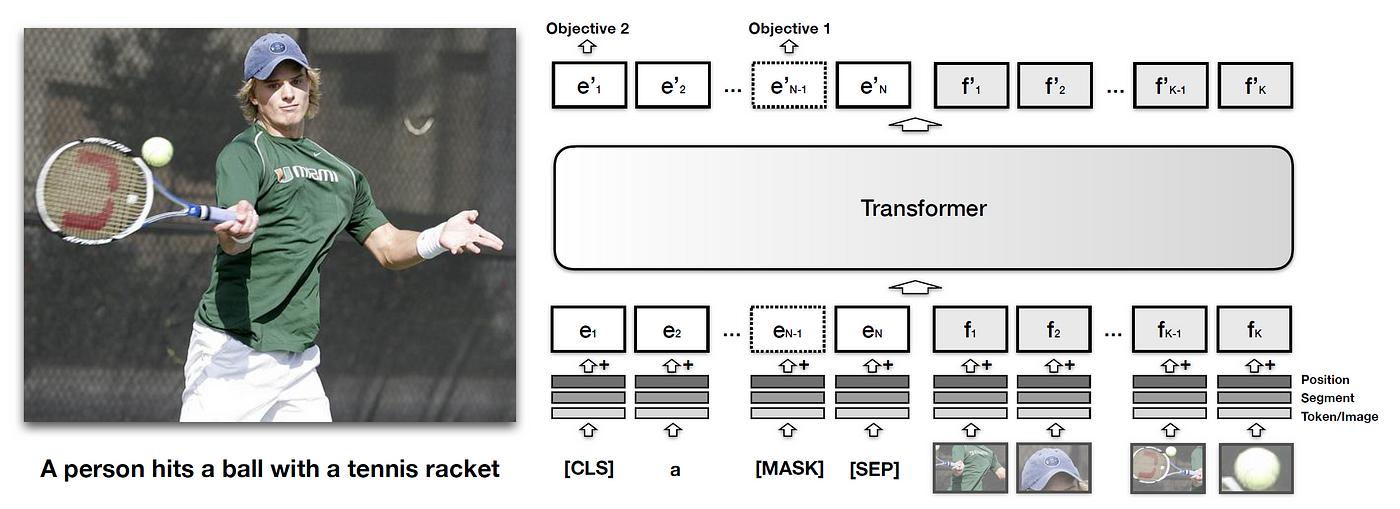
\includegraphics[scale=0.35]{imagens/visualBERT.png}
    \caption {Arquitetura do \textit{VisualBERT} \cite{VisualBERTArt}.}
\end{figure*}

\section{Multimodalidade}

A multimodalidade refere-se à capacidade de combinar e integrar múltiplas modalidades de comunicação, como texto, imagem, som, gestos e outros elementos sensoriais, para transmitir ou compreender informações de maneira mais rica e completa\footnote{\textit{What is Multimodal?} | \textit{University of Illinois Springfield}. Disponível em: \url{https://www.uis.edu/learning-hub/writing-resources/handouts/learning-hub/what-is-multimodal}. Acesso em: 12 jun. 2023.}. É a interação entre diferentes formas de representação e expressão que enriquece a comunicação e permite uma compreensão mais abrangente do conteúdo, permitindo uma comunicação mais rica e eficaz entre humanos e máquinas.

Ao lidar com a multimodalidade, os sistemas computacionais buscam interpretar e extrair informações de diferentes modalidades, permitindo que os usuários se envolvam de maneira mais natural e efetiva com a tecnologia. Essa abordagem é amplamente aplicada em áreas como processamento de linguagem natural, visão computacional, interação humano-computador e aprendizado de máquina, onde a combinação de modalidades permite uma compreensão mais rica e abrangente dos dados. Ao combinar informações de várias modalidades, é possível melhorar o desempenho de uma variedade de tarefas, resultando em soluções mais eficazes para uma ampla gama de desafios.

\section{Trabalhos Relacionados}

\subsection{Desafio dos Memes Odiosos (\textit{The Hateful Memes Challenge})} 

Este trabalho realizado pela equipe da Meta AI \cite{ArticleHatefulMemesChallenge2021} propôs um desafio para a classificação multimodal, com foco na detecção de discurso de ódio em memes multimodais. Fornecem modelos multimodais com diferentes níveis de sofisticação e ilustram como foi feita a criação do banco de dados com os memes odiosos e os memes categorizados como “confundidores benignos”. Esses confundidores foram adicionados ao conjunto de dados para aumentar a dificuldade do desafio, pois usam as mesmas imagens e frases que os memes odiosos, mas em contextos que não se enquadram como discurso de ódio. O objetivo deste desafio foi estimular a inovação e impulsionar o progresso no raciocínio e compreensão multimodal, que podem ter impactos positivos em várias tarefas e aplicações, ao mesmo tempo em que facilita o progresso da detecção de discurso de ódio e seu combate por meio de métodos automáticos.

\subsection{Detectando Discurso de Ódio em Memes Usando Abordagens de Aprendizado Profundo Multimodal} 

Os participantes do desafio proposto pela Meta IA adotaram uma abordagem que consistiu, primeiramente, em expandir o conjunto de treinamento por meio da busca por conjuntos de dados semelhantes na web. Em seguida, foram extraídas características das imagens utilizando algoritmos de detecção de objetos (\textit{Detectron}), o que permitiu aprimorar o modelo pré-treinado (\textit{VisualBERT}). Por fim, foi realizada a pesquisa de hiperparâmetros e aplicada a técnica de voto majoritário, atingindo 0,811 AUROC com uma precisão de 0,765 no conjunto de teste do desafio \cite{velioglu2020hateful}.